\section{Sequence wrench should be clickable}
\myref{fig:seq_wrench} shows how a guardian using the sequence tool views a sequence, as can be seen there is an image of the sequence thumbnail overlayed with a bin, representing a delete and a wrench.
The bin indicates that it is deletable, and deletes the sequence if tapped.
The wrench indicates that the sequence can be edited however unlike the bin this does nothing when tapped, despite doing so in other applications where the wrench is used.
When the wrench is tapped it should start the events that are included in editing, as it does if the thumbnail is tapped.
\begin{wrapfigure}{r}{0.3\textwidth}
    \centering
    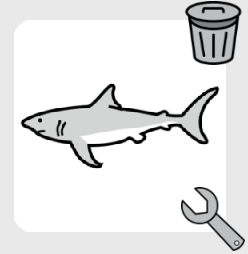
\includegraphics[width=0.3\textwidth]{figures/img/screenshots/sequence_pictogram.png} 
    \caption{A screenshot of a sequence thumbnail as viewed by a guardian.}
    \label{fig:seq_wrench} 
    \vspace{10pt}
\end{wrapfigure}
\bigskip
\noindent
In order to solve this problem firstly we go through the code looking for the implementation of both the bin and the wrench realising that these are both implemented as buttons.
These buttons will be refered to as the delete and the edit button respectively
The method which creates the button view, also calls the methods that provide their functionality, however no such method is called for the edit button.
An inspection of the code reveals that not only is no such metod called, but no such method exists despite the following comment on the method ``\/\/Adds a Delete \& Edit Icon to all Frames which deletes or edits the relevant Frame on click.''.